%! Author = gramic
%! Date = 15.03.24

% Preamble
\begin{flushleft}
    \subsubsection{yugabyteDB}
    \paragraph{Installation}
    Wähend der Installation des YugabyteDB Evaluations-Enviroment wurde festgestellt, das man zwei Varianten Installieren kann.
    YugabyteDB (Repository yugabyte) und YugabyteDB Anywhere (Repository yugawre):
    \begin{figure}[H]
        \centering
        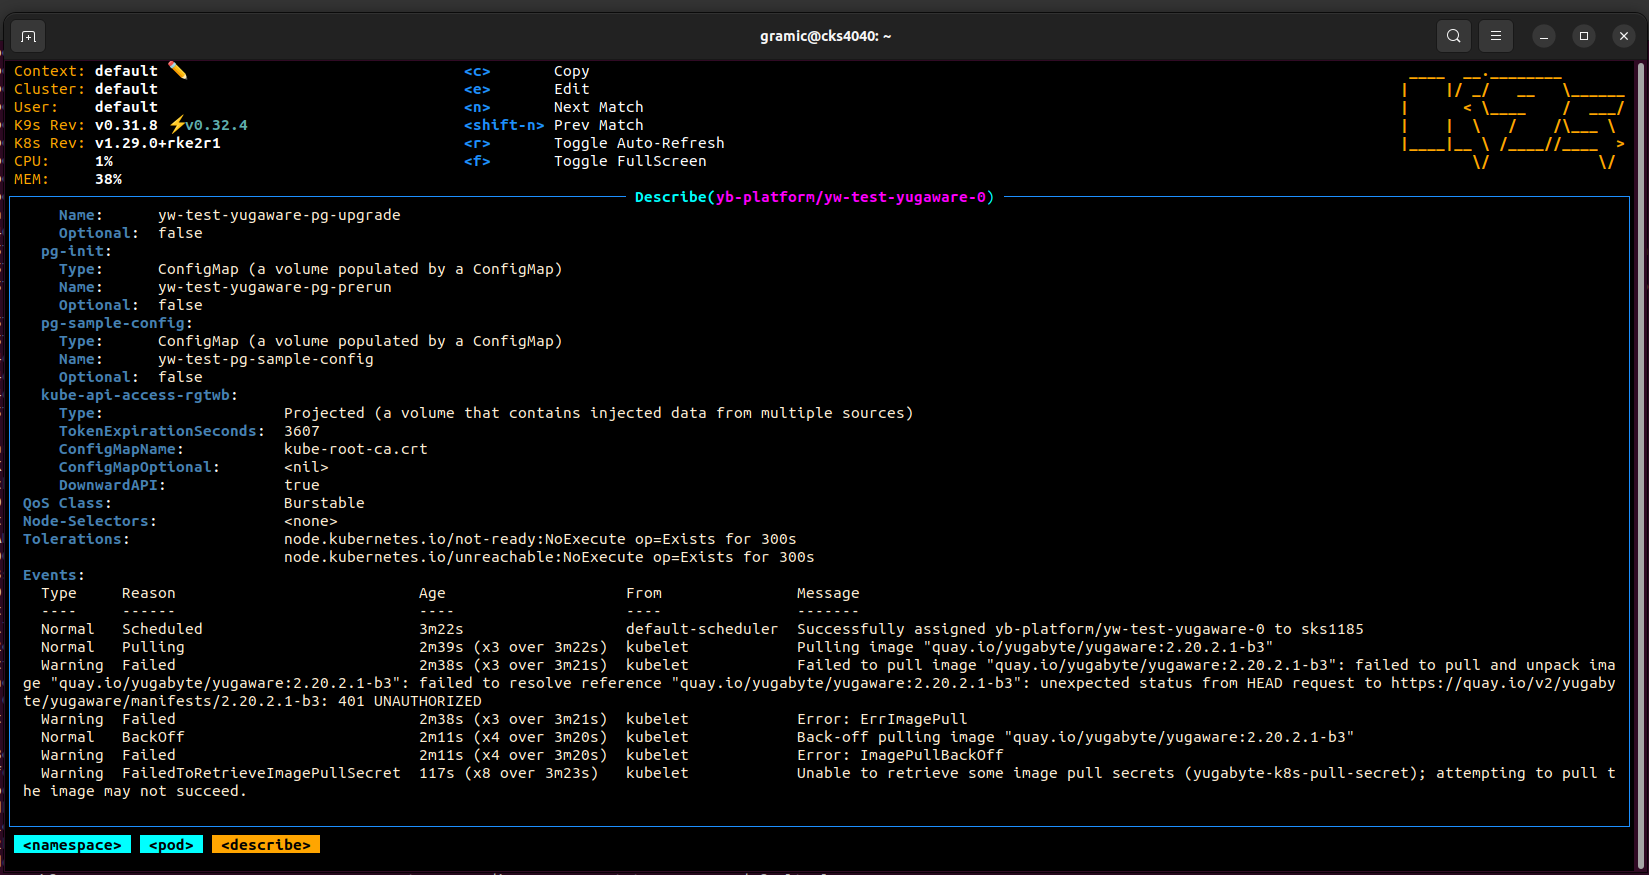
\includegraphics[width=1\linewidth]{source/implementation/evaluation/platforms/yugabytedb_pod_installation_subscription_interrup}
        \caption{yugabyteDB - Susbsription yugawre}
        \label{fig:yugabytedb_pod_installation_subscription_interrup}
    \end{figure}
\end{flushleft}
\begin{flushleft}
    Es stellte sich auch heraus, dass wenn man YugabyteDB 4 Cores pro Node zur Verfügung geben will (je zwei für den \texttt{master} und \texttt{tserver}),\\
    der Server mehr als 4 Cores haben muss.\\
    Andernfalls wird Kubernetes einen der beiden Pods nicht deployen, weil zuwenig Cores zur verfügung stehen.
\end{flushleft}
\begin{flushleft}
    Bei der konstelation \gls{rke2}, \Gls{Cilium} und \Gls{MetalLB}, muss nebst dem \texttt{IPAddressPool} auch ein \texttt{L2Advertisement} für den Pool gesetzt werden.\\
    Ansonsten kann die im YugabyteDB values.yaml gesetzte IP für den \texttt{tserver} von aussen nicht angesprochen werden:
    \lstset{style=gra_codestyle}
    \begin{lstlisting}[language=yaml, caption=metallb - Konfig YAML - Detail L2Advertisement,captionpos=b,label={lst:metallb-l2advertisement-setting},breaklines=true]
---
apiVersion: metallb.io/v1beta1
kind: L2Advertisement
metadata:
  name: l2adv
  namespace: metallb-system
spec:
  ipAddressPools:
  - distributed-sql
    \end{lstlisting}
    Dieses Problem ist schwer zu greifen und hat zwei Tage in Anspruch genommen, es zu Lösen.
    Die Vorschläge zum Lösen des Problems reichten von deakivieren von \texttt{kube-proxy} bis hin zu einer Migration zum \Gls{Cilium}-Loadb-Balancers.\\
    Mit diesem funktionierte dann nicht einmal mehr die Installation von yugabyteDB.\\
    Lösung brachte nur ein \texttt{GitHub}-Eintrag\cite{D4IZIEFN}, wo oben genannter Ansatz empfohlen wurde.
\end{flushleft}
\begin{flushleft}
    \paragraph{Konfiguration}
    Damit nicht der YugabyteDB Anywhere-Service installiert wird, muss das entsprechende Image gesetzt werden:
    \lstset{style=gra_codestyle}
    \begin{lstlisting}[language=yaml, caption=yugabyteDB - Helm Chart Manifest - Detail Image,captionpos=b,label={lst:yugabytedb-image-setting},breaklines=true]
...
Image:
  repository: "yugabytedb/yugabyte"
  tag: 2.20.2.1-b3
  pullPolicy: IfNotPresent
  pullSecretName: ""
...
    \end{lstlisting}

    Die StorageClass muss im \texttt{values.yaml} gesetzt werden, einmal für den \texttt{master} und einmal für den \texttt{tserver}
    \lstset{style=gra_codestyle}
    \begin{lstlisting}[language=yaml, caption=yugabyteDB - Helm Chart Manifest - Detail StorageClass,captionpos=b,label={lst:yugabytedb-storageclass-setting},breaklines=true]
...
storage:
  ephemeral: false  # will not allocate PVs when true
  master:
    count: 1
    size: 3Gi
    storageClass: "yb-storage"
  tserver:
    count: 1
    size: 3Gi
    storageClass: "yb-storage"
...
    \end{lstlisting}

    Dem node werden je 4 Cores zur verfügung gestellt.
    Zei für den \texttt{master} und zwei für den \texttt{tserver}.
    Beide erhalten 4GiB Memory:
    \lstset{style=gra_codestyle}
    \begin{lstlisting}[language=yaml, caption=yugabyteDB - Helm Chart Manifest - Detail Resources,captionpos=b,label={lst:yugabytedb-resources-setting},breaklines=true]
...
resource:
  master:
    requests:
      cpu: "1"
      memory: 2Gi
    limits:
      cpu: "1"
      ## Ensure the 'memory' value is strictly in 'Gi' or 'G' format. Deviating from these formats
      ## may result in setting an incorrect value for the 'memory_limit_hard_bytes' flag.
      ## Avoid using floating numbers for the numeric part of 'memory'. Doing so may lead to
      ## the 'memory_limit_hard_bytes' being set to 0, as the function expects integer values.
      memory: 2Gi
  tserver:
    requests:
      cpu: "1"
      memory: 4Gi
    limits:
      cpu: "1"
      ## Ensure the 'memory' value is strictly in 'Gi' or 'G' format. Deviating from these formats
      ## may result in setting an incorrect value for the 'memory_limit_hard_bytes' flag.
      ## Avoid using floating numbers for the numeric part of 'memory'. Doing so may lead to
      ## the 'memory_limit_hard_bytes' being set to 0, as the function expects integer values.
      memory: 4Gi
...
    \end{lstlisting}

    Die Shards, oder Tablets wie sie Yugabyte nennt, sollen auf allen drei Nodes repliziert werden:
    \lstset{style=gra_codestyle}
    \begin{lstlisting}[language=yaml, caption=yugabyteDB - Helm Chart Manifest - Detail Replika,captionpos=b,label={lst:yugabytedb-replica-setting},breaklines=true]
...
replicas:
  master: 3
  tserver: 3
  ## Used to set replication factor when isMultiAz is set to true
  totalMasters: 3
...
    \end{lstlisting}

    Wichtig ist auch, dass der \texttt{YSQL}-Dienst aktiv ist, damit PostgreSQL Abfragen abgesetzt werden können.\\
    Deshalb muss der Dienst aktiv sein und darf nicht deaktiviert werden:
    \lstset{style=gra_codestyle}
    \begin{lstlisting}[language=yaml, caption=yugabyteDB - Helm Chart Manifest - Detail Disable YSQL,captionpos=b,label={lst:yugabytedb-disableYsql-setting},breaklines=true]
...
# Disable the YSQL
disableYsql: false
...
    \end{lstlisting}

    Nun muss die Domain und die Service-Endpoints konfiguriert werden.\\
    Der Domainname bleibt vorerst \texttt{cluster.local} wie Default hinterlegt.\\
    Die Servicenamen und Ports werden nicht angetastet, wichtig ist die LoadBalancer-IP.\\
    Sie ist entsprechend der gewählten VirtualIP mit \texttt{10.0.20.106} zu setzen.

    \lstset{style=gra_codestyle}
    \begin{lstlisting}[language=yaml, caption=yugabyteDB - Helm Chart Manifest - Detail Domainname und Service-Endpoints,captionpos=b,label={lst:yugabytedb-domainname-serviceendpoints-setting},breaklines=true]
...
domainName: "cluster.local"

serviceEndpoints:
  - name: "yb-master-ui"
    type: LoadBalancer
    annotations: {}
    clusterIP: ""
    ## Sets the Service's externalTrafficPolicy
    externalTrafficPolicy: ""
    app: "yb-master"
    loadBalancerIP: ""
    ports:
      http-ui: "7000"

  - name: "yb-tserver-service"
    type: LoadBalancer
    annotations:
      metallb.universe.tf/loadBalancerIPs: 10.0.20.106
    clusterIP: ""
    ## Sets the Service's externalTrafficPolicy
    externalTrafficPolicy: ""
    app: "yb-tserver"
    loadBalancerIP: ""
    ports:
      tcp-yql-port: "9042"
      tcp-yedis-port: "6379"
      tcp-ysql-port: "5433"
...
    \end{lstlisting}
\end{flushleft}
\begin{flushleft}
    Beim Testen mit der höchsten Anzahl an Datensätzen zeigte sich, dass der \gls{local-path-provisioner} nicht sauber konfiguriert waren.\\
    Damit auf jedem Node die Persistence Volume Claims ausgeführt werden, müssen sie deklariert werden und in den StorageClass-Manifesten auch hinterlegt werden.\\
    Genauer muss in der \texttt{nodePathMap} folgende konfiguration vorgenommen werden:
\lstset{style=gra_codestyle}
\begin{lstlisting}[language=yaml, caption=local-path-provisioner nodePathMap,captionpos=b,label={lst:local-path-provisioner_nodePathMap},breaklines=true]
...
                "nodePathMap":[
                {
                        "node":"DEFAULT_PATH_FOR_NON_LISTED_NODES",
                        "paths":["<Lokaler Pfad>"]
                },
                {
                        "node":"<Nodename>",
                        "paths":["<Lokaler Pfad>"]
                },
...
\end{lstlisting}
    Hier ein Beispiel wie es mit den grossen Volumes aussieht:
\lstset{style=gra_codestyle}
\begin{lstlisting}[language=yaml, caption=local-path-provisioner nodePathMap Beispiel,captionpos=b,label={lst:local-path-provisioner_nodePathMap-exampl},breaklines=true]
...
                "nodePathMap":[
                {
                        "node":"DEFAULT_PATH_FOR_NON_LISTED_NODES",
                        "paths":["/srv/data/local-path-provisioner"]
                },
                {
                        "node":"sks1183",
                        "paths":["/srv/data/local-path-provisioner"]
                },
                {
                        "node":"sks1184",
                        "paths":["/srv/data/local-path-provisioner"]
                },
                {
                        "node":"sks1185",
                        "paths":["/srv/data/local-path-provisioner"]
                }
                ]
...
\end{lstlisting}
    Wird dies nicht gemacht, so wird auf den Default-Path geschrieben.\\
    Das ist zufällig und hat dann zur Folge, dass alle Volumes auf einem Node präsentiert werden.\\
    Was sehr schnell logischerweise dazu führt, dass zuwenig Diskspace vorhanden ist.\\
    Bei YugabyteDB kommt noch dazu, dass es zu Konflikten beim Schreiben von Blocks kommt.
\end{flushleft}
\begin{flushleft}
    Damit die Persistence Volumes sauber präsentiert werden, muss in der StorageClass die \texttt{nodeAffinity} gesetzt werden.\\
    Hier als Beispiel mit den Nodes \texttt{sks1183}, \texttt{sks1184} und \texttt{sks1185}:
\lstset{style=gra_codestyle}
\begin{lstlisting}[language=yaml, caption=yugabyteDB - StorageClass nodeAffinity,captionpos=b,label={lst:yugabytedb-storageclass_example},breaklines=true]
  nodeAffinity:
    required:
      nodeSelectorTerms:
      - matchExpressions:
        - key: kubernetes.io/hostname
          operator: In
          values:
          - sks1183
          - sks1184
          - sks1185
\end{lstlisting}
    \begin{warning}
        \textbf{hostPath}\\
        Der \texttt{hostPath} bei der StorageClass muss der gleiche sein, wie der Pfad im Node des nodePathMap von \gls{local-path-provisioner}.
        Auch sollten die Pfade auf allen Nodes gleich sein.
    \end{warning}
\end{flushleft}
\begin{flushleft}
    Die Problematik mit dem \texttt{nodePathMap} und der \texttt{nodeAffinity} auf der StorageClass hat auch rund zwei Arbeitstage in Anspruch genommen.
\end{flushleft}